% !TEX program = pdflatex

\RequirePackage[l2tabu, orthodox]{nag}
\documentclass[10pt]{article}

% GEOMETRY
\usepackage[paper=letterpaper,
			left=1.5in,               
			right=1.5in,
			top=1.0in,
			bottom=1.0in,
			]{geometry}

% FIGURES
\usepackage{caption}
\usepackage{subcaption}

% FONTS
\usepackage[T1]{fontenc}
\usepackage{garamondx}
\usepackage[garamondx,cmbraces]{newtxmath}

% COLORS
\usepackage[usenames,dvipsnames,svgnames]{xcolor}

% USEFUL
\usepackage{microtype}
\usepackage[parfill]{parskip} 
\usepackage{cleveref}
\usepackage{graphicx}

\usepackage{listings}

\lstset{ %
  basicstyle=\scriptsize\ttfamily,        % the size of the fonts that are used for the code
  breakatwhitespace=false,         % sets if automatic breaks should only happen at whitespace
  breaklines=true,                 % sets automatic line breaking
  frame=single,                    % adds a frame around the code
  keepspaces=true,                 % keeps spaces in text, useful for keeping indentation of code (possibly needs columns=flexible)
  tabsize=2,                       % sets default tabsize to 2 spaces
}


\title{ResMap Manual\break {\normalsize\texttt{[version 1.1.2]}}}
\author{Alp Kucukelbir, Fred Sigworth, Hemant Tagare}
\date{October 29, 2013}

\begin{document}
\maketitle

\tableofcontents

\section{Purpose}
Local Resolution Map (ResMap) is a Python (NumPy/SciPy) application with a Tkinter GUI and a command-line interface. It is a software package for computing the local resolution of 3D density maps studied in structural biology, primarily electron cryo-microscopy (cryo-EM).

\newpage

\section{Downloading \& Installing}
\label{downloadAndInstall}
Binaries for Windows, Mac, and Linux, along with the Python source code is available on SourceForge:
\begin{center}
	\textcolor{NavyBlue}{\texttt{http://resmap.sourceforge.net}}
\end{center}

Please choose your operating system and SourceForge should automatically provide you with the latest binary for your platform.

The binaries have been packaged using PyInstaller\footnote{http://www.pyinstaller.org/} and were tested on:
\begin{center}
	\textbf{Windows:} 7 and 8 \quad	\textbf{Mac:} 10.6+ \quad \textbf{Linux:} Fedora 14, CentOS 6
\end{center}

\textcolor{RedOrange}{\textbf{NOTE:}} Mac and Linux users may need to change the permissions of the downloaded binary to launch the program. To do so, please execute the following command from the terminal,
\begin{center}
	\textcolor{NavyBlue}{\texttt{chmod +x ResMap-1.1.2-distrib}}
\end{center}
where you should replace the name of the binary with the exact file that you downloaded.

You may also download the source files (Python) and run them using your own Python setup. You will need to install:
\begin{center}
	\textbf{Python:} 2.7+ \quad	\textbf{NumPy:} 1.6+ \quad \textbf{SciPy:} 0.12+ \quad \textbf{Matplotib:} 1.2+
\end{center}

\section{Launching the Program (Graphical Mode)}
To run the program in graphical mode, in Windows simply double click the binary, while in Mac and Linux, execute the following command from the terminal 
\begin{center}
	\textcolor{NavyBlue}{\texttt{./ResMap-1.1.2-distrib}}
\end{center}

You should see a graphical user interface (GUI) show up, as shown in \Cref{fig:gui_singleVolume}.
\begin{figure}[!h]
\centering
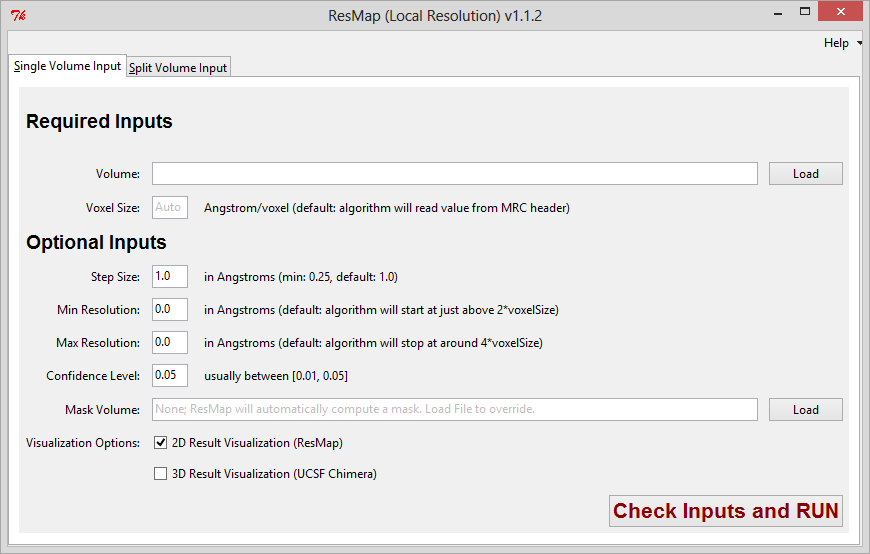
\includegraphics[width=4in]{img/gui_singleVolume_112.png}
\caption{ResMap Graphical User Interface (shown on Windows 8 here)}
\label{fig:gui_singleVolume}
\end{figure}

\textcolor{RedOrange}{\textbf{NOTE:}} The first time you launch ResMap, it may take a while for the GUI to appear. Subsequent launches of ResMap should not suffer from this delay.

\section{Launching the Program (Command Line Mode)}
To run the program in command line mode, open a command line prompt or terminal and change your directory to where you downloaded the ResMap binary. The command line interface is presented below. 

\medskip

\begin{lstlisting}
Usage: 
  ResMap.py [(--noguiSingle INPUT)] [--vxSize=VXSIZE]
            [--pVal=PVAL]
            [--minRes=MINRES] [--maxRes=MAXRES] [--stepRes=STEPRES]
            [--maskVol=MASKVOL]
            [--vis2D] [--launchChimera] [--noiseDiag]
  ResMap.py [(--noguiSplit INPUT1 INPUT2)] [--vxSize=VXSIZE]
            [--pVal=PVAL]
            [--minRes=MINRES] [--maxRes=MAXRES] [--stepRes=STEPRES]
            [--maskVol=MASKVOL]
            [--vis2D] [--launchChimera] [--noiseDiag]

NOTE: INPUT(s) is/are mandatory

Arguments:
  INPUT(s)            Input volume(s) in MRC format

Options:
  --noguiSingle       Run ResMap for Single Volumes in command-line mode
  --noguiSplit        Run ResMap for Split Volumes in command-line mode
  --vxSize=VXSIZE     Voxel size of input map (A) [default: 0.0]
  --pVal=PVAL         P-value for likelihood ratio test [default: 0.05]
  --minRes=MINRES     Minimum resolution (A) [default: 0.0]       
  --maxRes=MAXRES     Maximum resolution (A) [default: 0.0]      
  --stepRes=STEPRES   Step size (A) [default: 1.0]                
  --maskVol=MASKVOL   Mask volume                                 
  --vis2D             Output 2D visualization
  --launchChimera     Attempt to launch Chimera after execution
  --noiseDiag         Run and show noise diagnostics
  -h --help           Show this help message and exit
  --version           Show version. 
\end{lstlisting}

\section{Single Volume vs.~Split Volume Mode}
\subsection{Single Volume Input}
ResMap is designed to work by taking a single volume as input. It will isolate the background voxels in the map to estimate relevant noise statistics. This is a reliable and convenient way of using ResMap.

\subsection{Split Volume Input}
ResMap has now been extended to work on split volumes, too. Split volumes are needed to compute FSC plots and therefore many users may find practical value in re-using these volumes that they may have handy. In split volume mode, ResMap will compute a difference map by subtracting the split volumes from each other to estimate relevant noise statistics. Note that your split volumes \textbf{must be aligned} or else artifacts will appear in the difference map and ResMap results may not make any sense.

\section{Understanding the Inputs}
\subsection{Input Volume(s)}
\label{inputVolProperties}
ResMap can read and write MRC/CCP4 volumes. It assumes the volumes are cubic, with equal number of voxels along all three dimensions.

ResMap \textcolor{BrickRed}{\textbf{absolutely needs}} the input volume(s) to have these properties
\begin{enumerate}
	\item The particle must be centered in the volume. (Helical particles are not well supported, yet.)
	\item The background must not been masked out (e.g.~by a routine, like Bsoft's \texttt{blocres}).
\end{enumerate}

ResMap \textcolor{BrickRed}{\textbf{prefers}}, but does not \textcolor{BrickRed}{\textbf{necessitate}} the input volume(s) to have these properties
\begin{enumerate}
	\item The volume has \textbf{not} been filtered in any way (low-pass filtering, etc.)
	\item The volume has a realistic noise spectrum. This is sometimes obtained by so-called amplitude correction. While a similar effect is often obtained by B-factor sharpening, please make sure that the spectrum does not blow up near Nyquist.
\end{enumerate}
\Cref{fig:inputs} depicts common cases of preferred, valid and invalid input volumes.

\begin{figure}[!ht]
	\centering
	\begin{subfigure}[b]{0.4\textwidth}
	        \centering
	        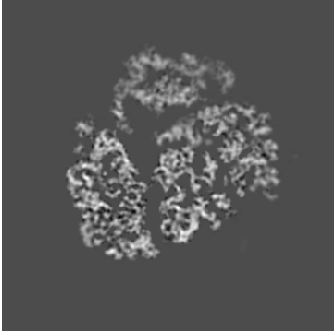
\includegraphics[width=\textwidth]{img/2_2239.png}
	        \caption{\textcolor{BrickRed}{\textbf{INVALID:}} This map has been masked by Bsoft's \texttt{blocres} routine (EMD-2239). ResMap cannot operate on this map.\newline}
	\end{subfigure}
	\qquad %add desired spacing between images, e. g. ~, \quad, \qquad etc.
	  %(or a blank line to force the subfigure onto a new line)
	\begin{subfigure}[b]{0.4\textwidth}
	        \centering
	        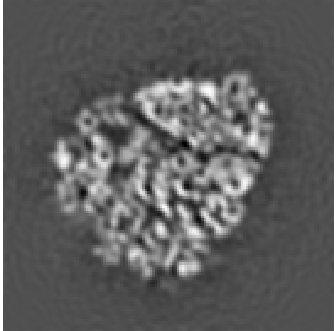
\includegraphics[width=\textwidth]{img/1_5562.png}
	        \caption{\textcolor{RedOrange}{\textbf{NOT IDEAL:}} This map has been low pass filtered (EMD-5562). ResMap will attempt to run, but may fail.\newline}
	\end{subfigure}
	%add desired spacing between images, e. g. ~, \quad, \qquad etc.
	%(or a blank line to force the subfigure onto a new line)
	\begin{subfigure}[b]{0.4\textwidth}
	        \centering
	        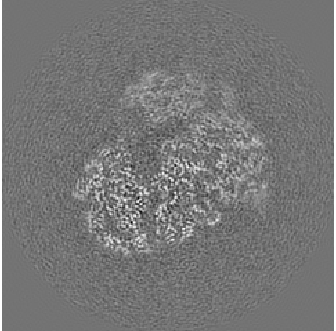
\includegraphics[width=\textwidth]{img/4_2275.png}
	        \caption{\textcolor{RedOrange}{\textbf{NOT IDEAL:}} This map has been B-factor sharpened (EMD-2275). ResMap will attempt to run, but may fail. \newline}
	\end{subfigure}
	\qquad %add desired spacing between images, e. g. ~, \quad, \qquad etc.
	  %(or a blank line to force the subfigure onto a new line)
	\begin{subfigure}[b]{0.4\textwidth}
	        \centering
	        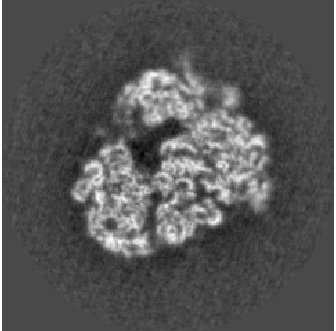
\includegraphics[width=\textwidth]{img/3_sjors.png}
	        \caption{\textcolor{LimeGreen}{\textbf{PREFERRED:}} This map has not been processed (raw version of EMD-2275). ResMap run reliably on this map. \newline}
	\end{subfigure}
	\caption{Input volume cases.}
	\label{fig:inputs}
\end{figure}

Note that some the above properties may exclude some of the maps already uploaded to the EMDB. While this may seem like a limitation, we were really happy to talk to Catherine Lawson at the 2013 Gordon Conference and some of the other folks involved in the EM Validation Task Force. It seems like there is a move towards encouraging the upload of \emph{unfiltered} maps to the EMDB. This way the real data are posted online and statistical computations, like those performed in ResMap, can be conducted on maps publicly available on the EMDB.

\subsection{Min, Max Resolution and Step Size}
These fields are provided to accelerate computation if you are only interested in analyzing a specific resolution range. It is usually a good idea to provide a maximum resolution value to save time. Another way to save computation is to provide a larger step size.

\subsection{Confidence Level}
This is the p-value of the statistical hypothesis test on which ResMap is based on. It is customarily set to $0.05$ although you are welcome to reduce it (e.g.~$0.01$) if you would like to obtain a more conservative result. Empirically, ResMap results are not much affected by the p-value.

\subsection{Mask Volume}
It is not necessary to provide ResMap with a mask volume. The algorithm will attempt to estimate a mask volume by low-pass filtering the input volume and thresholding it using a heuristic procedure. 

If the automated procedure does not work well for your particle, you may provide a mask volume that matches the input volume in size and format. The mask volume should be a binary volume with zero (0) denoting the background/solvent and some positive value (0+) enveloping the particle.

\section{Using the ResMap Pre-Whitening Interface (Beta)}
ResMap as of \texttt{[v.1.0.7]} provides an interactive graphical pre-whitening tool (\Cref{fig:prewhitening}). The tool was significantly re-vamped in \texttt{[v.1.1.0]} with many performance updates. 

Specifically, ResMap now offers two different pre-whitening modes: one for reasonably sized volumes and another for larger volumes. Descriptions are provided in the terminal as ResMap is running. In both modes, the usage, as described below, is the same:

\begin{figure}[!h]
\centering
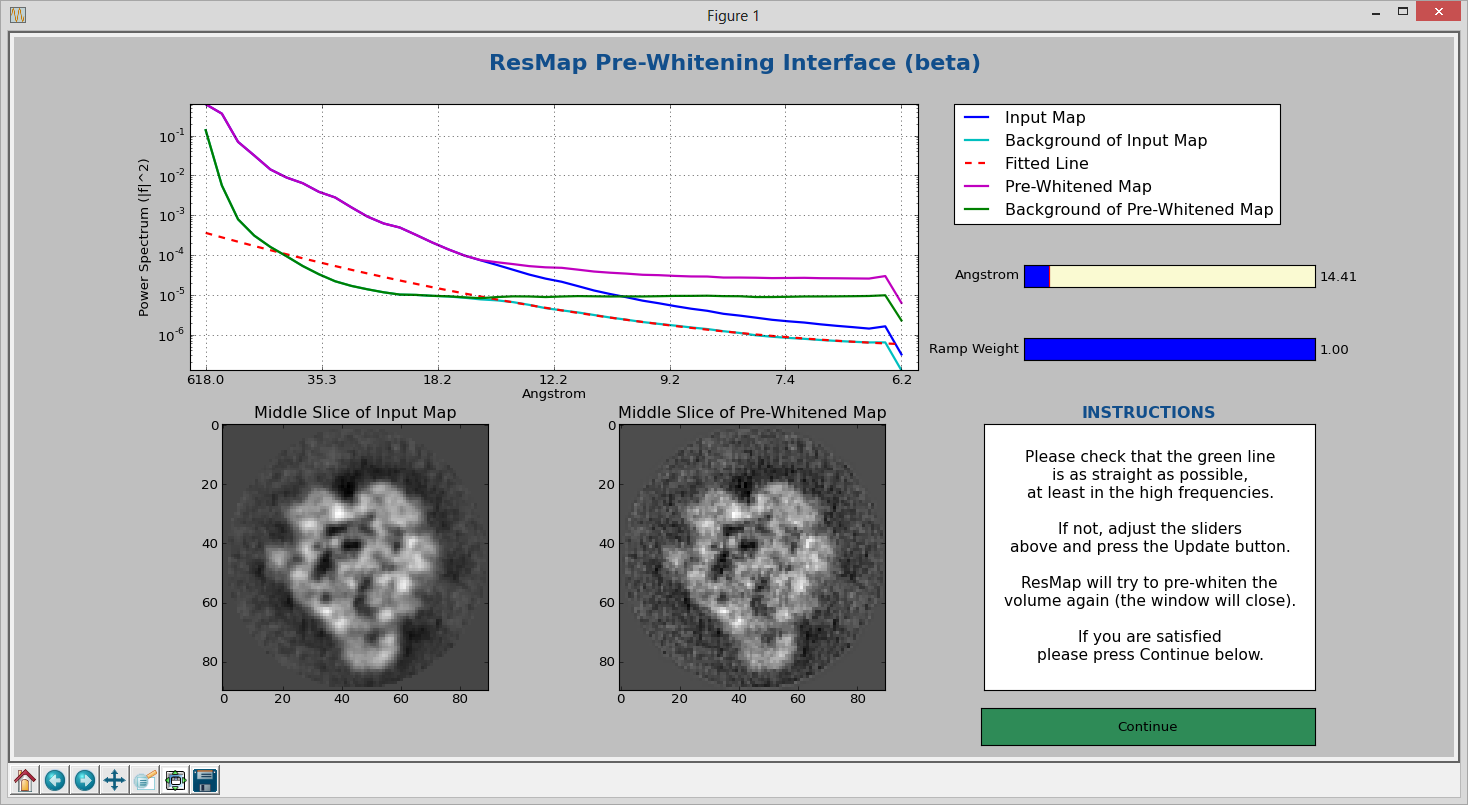
\includegraphics[width=5in]{img/gui_preWhitening.png}
\caption{ResMap Pre-Whitening Interface as seen on a reasonably sized volume. The passband has been set adjusted to 14.41\AA{} to obtain a flat Green curve.}
\label{fig:prewhitening}
\end{figure}

ResMap will attempt to pre-whiten your input volume(s) in the following way:
\begin{enumerate}
	\item Plot the power spectrum of the input volume [Blue]
	\item Plot the power spectrum of the background (via soft mask or difference map) [Cyan]
	\item Fit a polynomial (up to order 2) to the Cyan curve, between a passband (default 10\AA{}) and Nyquist [Dotted Red]
	\item Pre-whiten the volume by correcting for this slope (using a ramp weight between 0 and 1)
	\item Plot the power spectrum of the pre-whitened volume (Magenta)
	\item Plot the power spectrum of the pre-whitened background (Green)
	\item If all goes well, the Green curve should be fairly flat, at least in the high frequencies.
	\item If not, allow the user to adjust the passband and ramp weight to hopefully obtain a flat Green curve.
\end{enumerate}

\textcolor{RedOrange}{\textbf{NOTE:}}  The filtering is not instant! It involves a few Fourier transforms and such. If you adjust the passband or ramp weight, please give it some time to re-compute the pre-whitening.

\textcolor{RedOrange}{\textbf{NOTE:}} If the pre-whitening causes unexpected problems, simply set the ramp weight to 0. This should effectively by-pass the pre-whitening routine. Please also notify the authors as we would like to make this tool as robust as possible.

\section{Visualizing the Outputs}
ResMap will output an MRC/CCP4 volume with the same filename as the input volume, but with \texttt{\_resmap.map} appended to the end. In the split volume mode, it will use the filename of the first volume. Resmap will also write out a UCSF Chimera script for 3D visualization with the same filename as the input volume, but with \texttt{\_resmap\_chimera.cmd} at the end. 

ResMap now offers two ways of visualizing the results:
\begin{description}
	\item[2D:] It is useful to look at individual slices of the ResMap volume, as this provides a detailed view into the varying resolution in your map. ResMap now has the option of outputting some slices through the map after execution. ResMap will also output a histogram of the assigned resolutions. Select this option either via the command-line interface or GUI to enable a 2D visualization to appear after ResMap has finished computing.

	\textcolor{RedOrange}{\textbf{NOTE:}} You can save the 2D figures in a variety of formats: PNG, TIFF, JPEG, PS, EPS, SVG, PDF, and \LaTeX{} PGF.

	\item[3D:] ResMap now, thanks to the help of Tom Goddard from the Chimera team, outputs a Chimera script along with the resolution map. ResMap offers an option to automatically launch this script into Chimera after ResMap has finished its computations. The script makes use of Chimera's \texttt{Tools > Volume Data > Surface Color}\footnote{http://www.cgl.ucsf.edu/chimera/docs/ContributedSoftware/surfcolor/surfcolor.html} to color the surface of your input map with the results of ResMap, and animate a slice as it goes through a low-pass filtered contour of the input volume. 
\end{description}

\begin{figure}[!h]
\centering
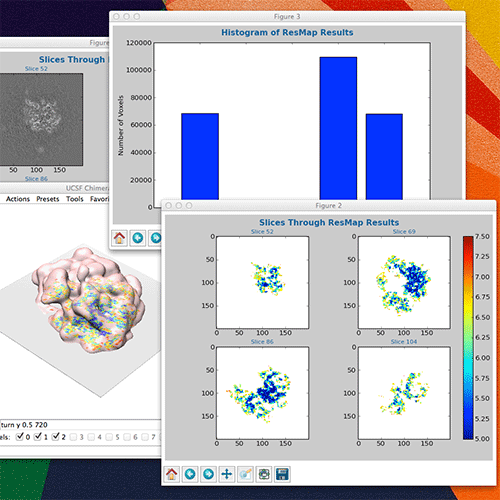
\includegraphics[width=4in]{img/viz.png}
\caption{ResMap 2D and 3D Visualization Results}
\end{figure}

% \begin{figure}[!h]
% \centering
% 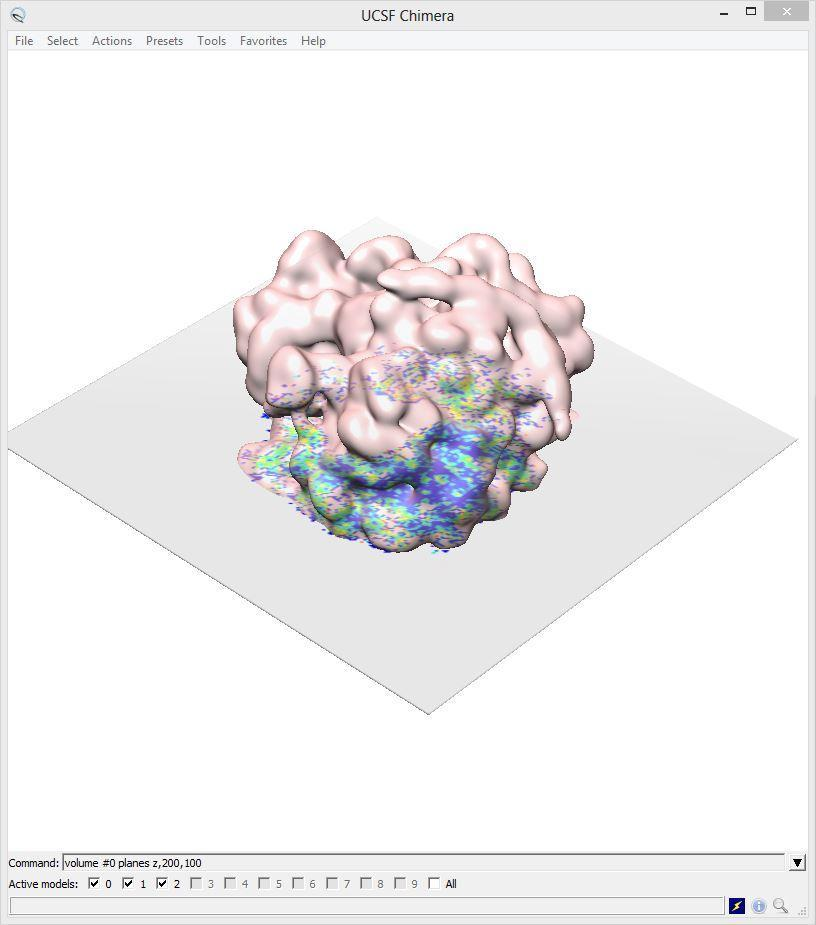
\includegraphics[width=3in]{img/chimeraViz.JPG}
% \caption{ResMap Results Visualized in UCSF Chimera}
% \end{figure}

\clearpage
\section{Troubleshooting}

\textcolor{RedOrange}{\emph{The binary does not work!}}
\begin{quote}
	Please contact the authors. If you are willing, please consider installing Python and the dependencies noted in \Cref{downloadAndInstall} and running ResMap from the source. 
\end{quote}

\textcolor{RedOrange}{\emph{The results are over-/under-estimating the resolution!}}
\begin{quote}
	Please check that the power spectrum after the pre-whitening looks reasonable. Please also check that your input volume satisfies the requirements in \cref{inputVolProperties}. If the numbers still do not make sense, please contact the authors.
\end{quote}

\textcolor{RedOrange}{\emph{Why can't ResMap do X?}}
\begin{quote}
	We would love to hear your suggestions! Please contact the authors.
\end{quote}

\section{Citing}
If you use ResMap, we kindly ask that you use the following citation:

\begin{quote}
	A.~Kucukelbir, F.J.~Sigworth, H.D.~Tagare, \textcolor{BrickRed}{Quantifying the Local Resolution of Cryo-EM Density Maps}, \textcolor{OliveGreen}{\emph{Nature Methods}}, In Press 2013.
\end{quote}

\section{Changelog}
\begin{description}
	\item[1.1.2] Automatic voxel spacing grab from MRC header, GUI updates.
	\item[1.1.0] Major ResMap update: new split volume mode, updated pre-whitening interface, and overal much faster pre-whitening implementation.
	\item[1.0.8] Bug fixes.
	\item[1.0.7] ResMap now provides a pre-whitening interface and accepts an ad-hoc variance estimate.
	\item[1.0.6] ResMap now also supports a command line interface on all platforms (Mac/Windows/Linux).
	\item[1.0.5] ResMap will out produce a USCF Chimera script and attempt to launch it after execution. Many thanks to Tom Goddard for the Chimera script and the advice to make this work!
	\item[1.0.4] ResMap will now detect low-pass filtered inputs and downsample the volume accordingly during calculations. Also, 2D graphical output option added.
	\item[1.0.3] Low-pass filtering detection subroutine implemented.
	\item[1.0.2] Bug fixes.
	\item[1.0.1] Mask volume bug fixed.
	\item[1.0.0] Initial release.
\end{description}

\end{document}